\Cref{sec:photon_selection} introduced the best-photon candidate strategy, 
as well as selection to suppress events 
where the photon is misidentified or originates in sources different than \BtoXsgamma.
However, as was seen before in, for example. \Cref{fig:photon_reco_candidates_bplus,fig:photon_reco_candidates_bzero},
\epem\ra\qqbar events provide the vast majority of photon candidates.
Therefore, a dedicated event-selection for this type of background was devised.
It takes advantage of  different event topologies expected for $\FourS\to\qqbar$ and $\epem\ra\qqbar$ events.
Loosely speaking, events where a $\FourS\to\BB$ decay is present tend to be more `spherical', when compared with $\epem\ra\qqbar$ events that exhibit a `jet-like' distribution.
This is related to the fact that \epem collissions at $B$ dactory experiments have just enough energy to produce a $B$ pair almost at rest, which means that its decays products, on average, tend to be distributed uniformly in polar and azimuthal angle.
On the other hand, light-quark pairs, produced in \epem collision events, also gain a substantial amount of back-to-back momentum which tends to spread their decay products. 
The schematic idea of this is shown in \Cref{fig:continuum_schematic}.
This section will provide an in-depth discussion on how the discrimination between \BtoXsgamma and continuum is achieved using a \BDT.

\begin{figure}[htbp!]
    \centering
    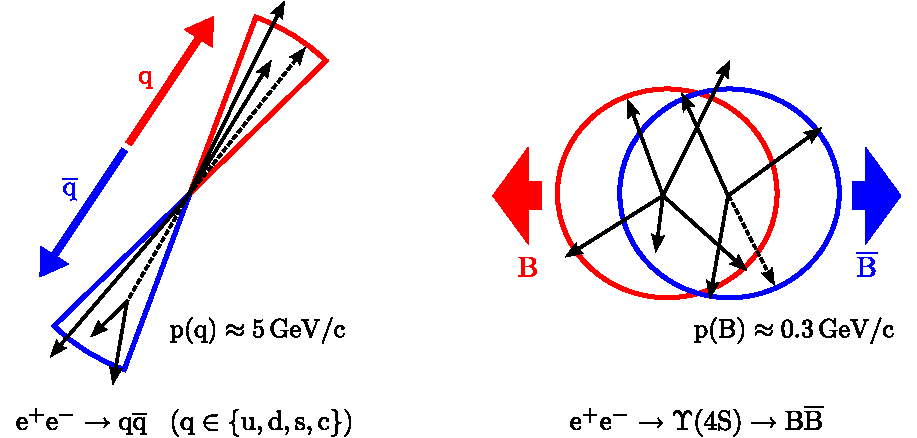
\includegraphics[width=0.6\textwidth]{figures/continuum_suppression/figure_continuum_suppression_event_shapes.pdf}
    \caption{\label{fig:continuum_schematic} Schematic illustration of continuum and \BB events created after an \epem collision in $B$ factories.
    Events where a $B$ meson is produced are generally more spherical, due to the fact that \FourS is produced at rest and its decays products tend to not have a preferred direction.
    Typical momenta of light-quark and \BB mesons are shown.
    The specific directions shown are illustrative only. 
    }
\end{figure}

\subsection{Training event pre-selection}\label{sec:preselection}

Before a \BDT is trained, it is generally desirable to prepare the datasets such that the classifier 
is able to learn based on relevant data.
Such data preprocessing will be performed based on variables described in \Cref{sec:photon_selection}.
The classifier will then be trained on the reduced dataset

In order to find optimal selections, a figure-of-merit study is performed for each observable.
Two figure of merit options were considered for this analysis, a more standard figure-of-merit $\mathrm{FOM}_1$:
\begin{equation}\label{eq:soversqrtsplusb}
    \mathrm{FOM}_1 = \frac{\mathsf{S}}{\sqrt{\mathsf{S}+\mathsf{B}}},
\end{equation}
and $\mathrm{FOM}_2$ defined in Ref.\cite{Punzi:2003bu} (often referred to as `Punzi' figure-of-merit):
\begin{equation}\label{eq:punzi_fom}
    \mathrm{FOM}_2 = \frac{\mathsf{S}}{\mathsf{S}_0} \frac{1}{\frac{3}{2}+\sqrt{\mathsf{B}}}.
\end{equation}
In both equations, $\mathsf{S}$ is the number of signal events after selection, 
$\mathsf{B}$ is the number of background events after selection, 
and $\mathsf{S}_0$ is the number of signal events before selection.
Although \Cref{eq:punzi_fom} was derived with search-like analyses in mind, 
it is utilised in this analysis to minimise signal model dependancy: the ratio $\mathsf{S}/\mathsf{S}_0$ present in the definition reduces out many model-dependant effects.

For each figure of merit calculation, background events ($\mathsf{B}$) are calculated based on generic \MC,
whereas signal events, $\mathsf{S}$, are calculated based on signal \MC, to ensure a high statistics sample.
In the case of \Cref{eq:soversqrtsplusb}, an appropriate scaling for $\mathsf{S}$ is also used.
Each dataset has duplicate tag-candidate events randomly removed, by picking a random tag-side candidate.
Each figure of merit is then calculated for 200 equally spaced selections in the target observable.
The maximum figure-of-merit point is taken as the optimal pre-selection for each of the variables.
This procedure is shown for $\mathrm{FOM}_2$ in \Cref{fig:selection_optimisations}.
Results for $\mathrm{FOM}_1$ are used as a cross-check for $\mathrm{FOM_2}$ but turn out to be consistent.
Equivalent procedure for $\mathrm{FOM}_1$ is shown in \Cref{sec:appendix_sqrtsplusb_optimisation}.
The resulting optimal selections are also shown in the Figures.

\begin{figure}[htbp!]
    \centering
    \subcaptionbox{\label{fig:bp_zmva_optimisation}}{
            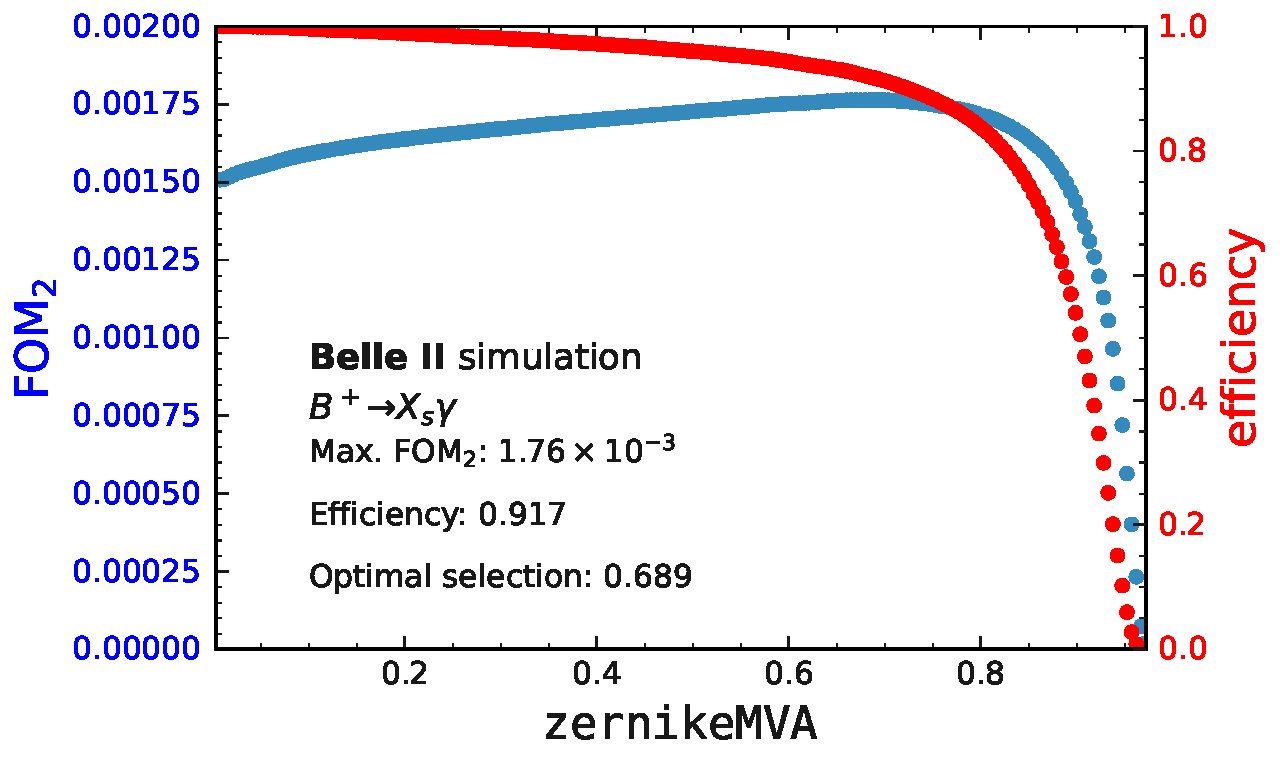
\includegraphics[width=0.3\textwidth]{figures/continuum_suppression/Bp_zernikeMVA_optimisation_punzi.pdf}
        }
    \subcaptionbox{\label{fig:bp_piveto_optimisation}}{
            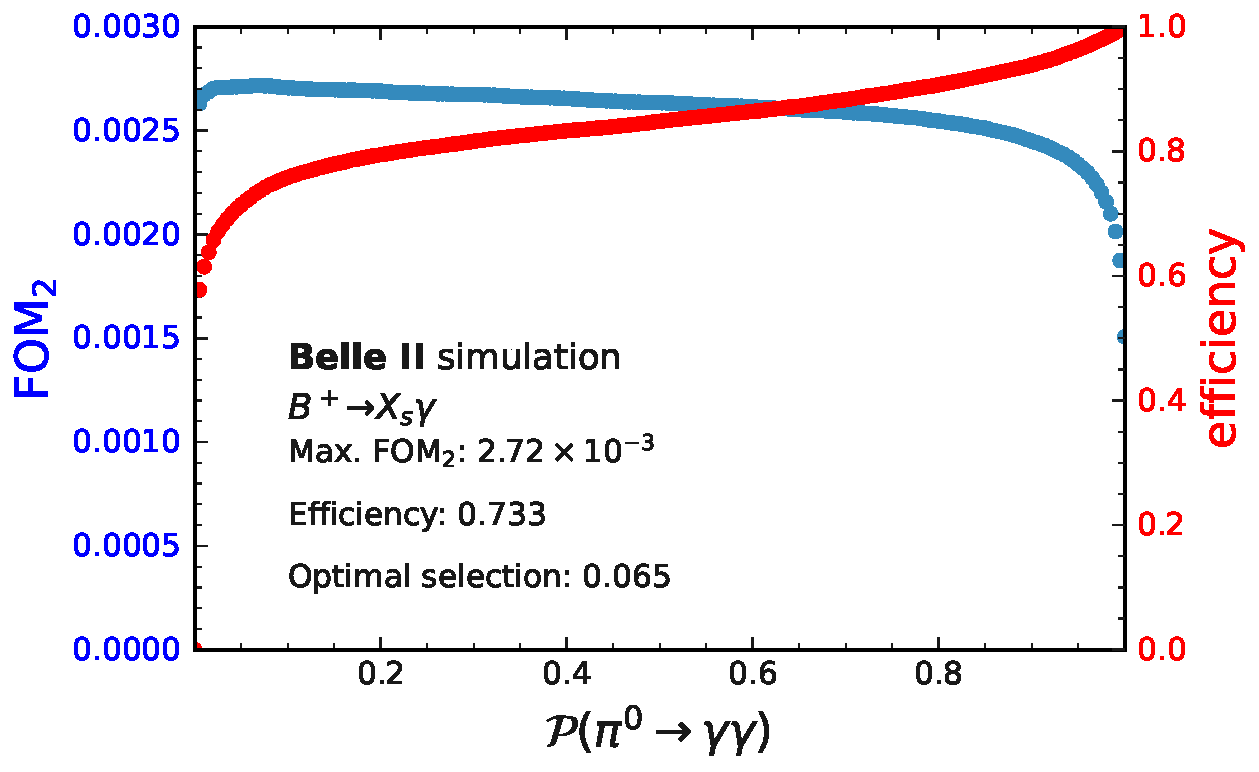
\includegraphics[width=0.3\textwidth]{figures/continuum_suppression/Bp_piVeto_optimisation_punzi.pdf}
        }
    \subcaptionbox{\label{fig:bp_etaveto_optimisation}}{
            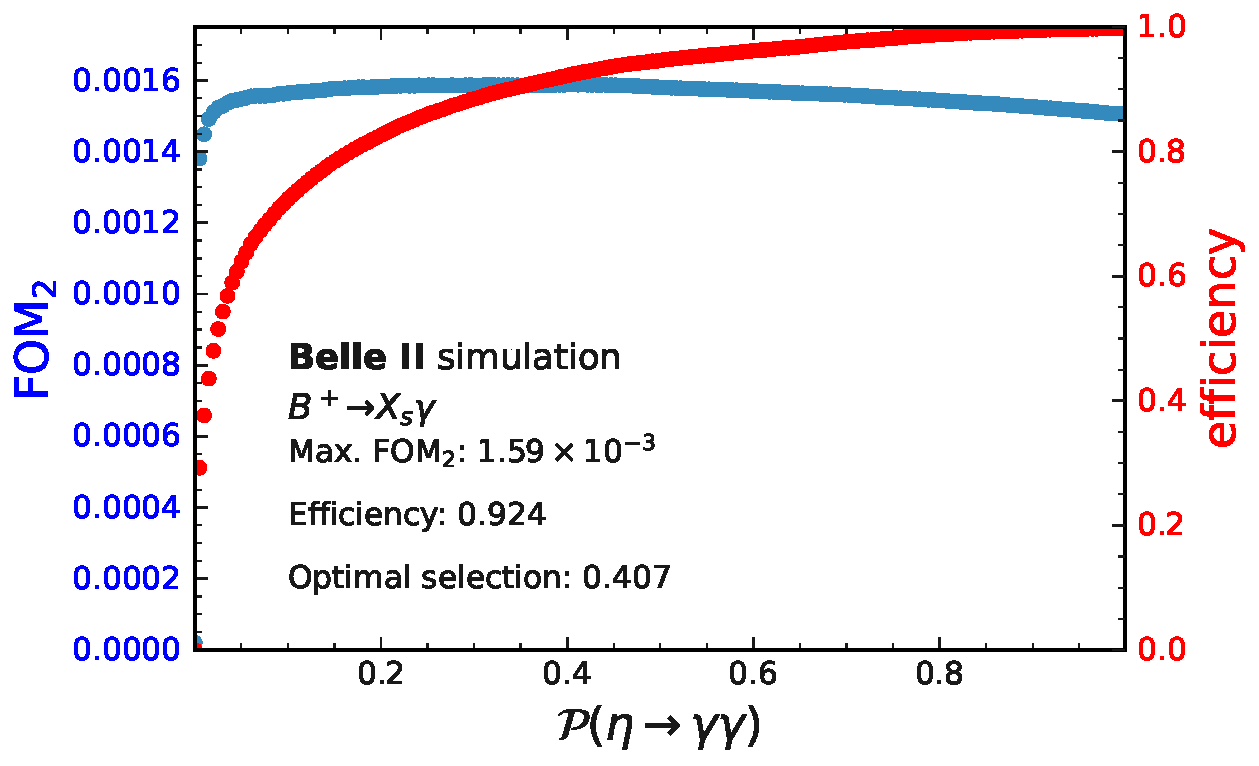
\includegraphics[width=0.3\textwidth]{figures/continuum_suppression/Bp_etaVeto_optimisation_punzi.pdf}
        }
    \subcaptionbox{\label{fig:bz_zmva_optimisation}}{
            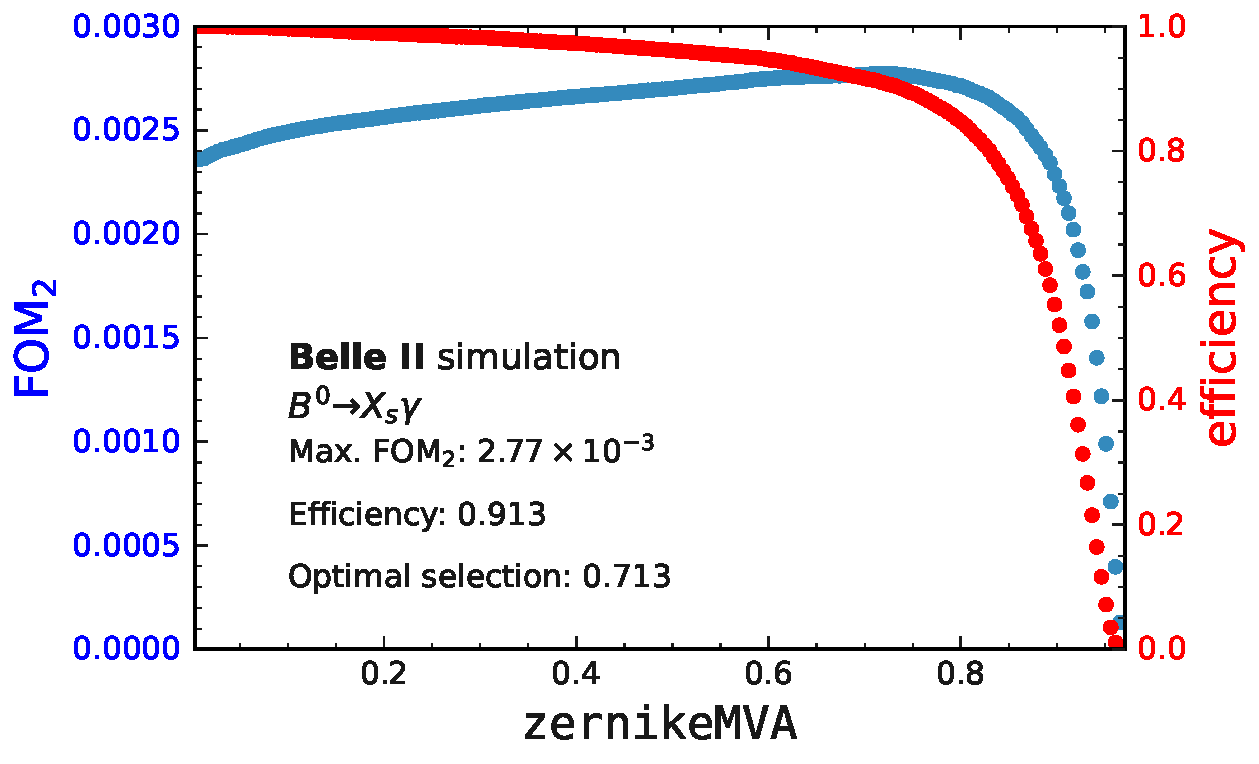
\includegraphics[width=0.3\textwidth]{figures/continuum_suppression/Bz_zernikeMVA_optimisation_punzi.pdf}
        }
    \subcaptionbox{\label{fig:bz_piveto_optimisation}}{
            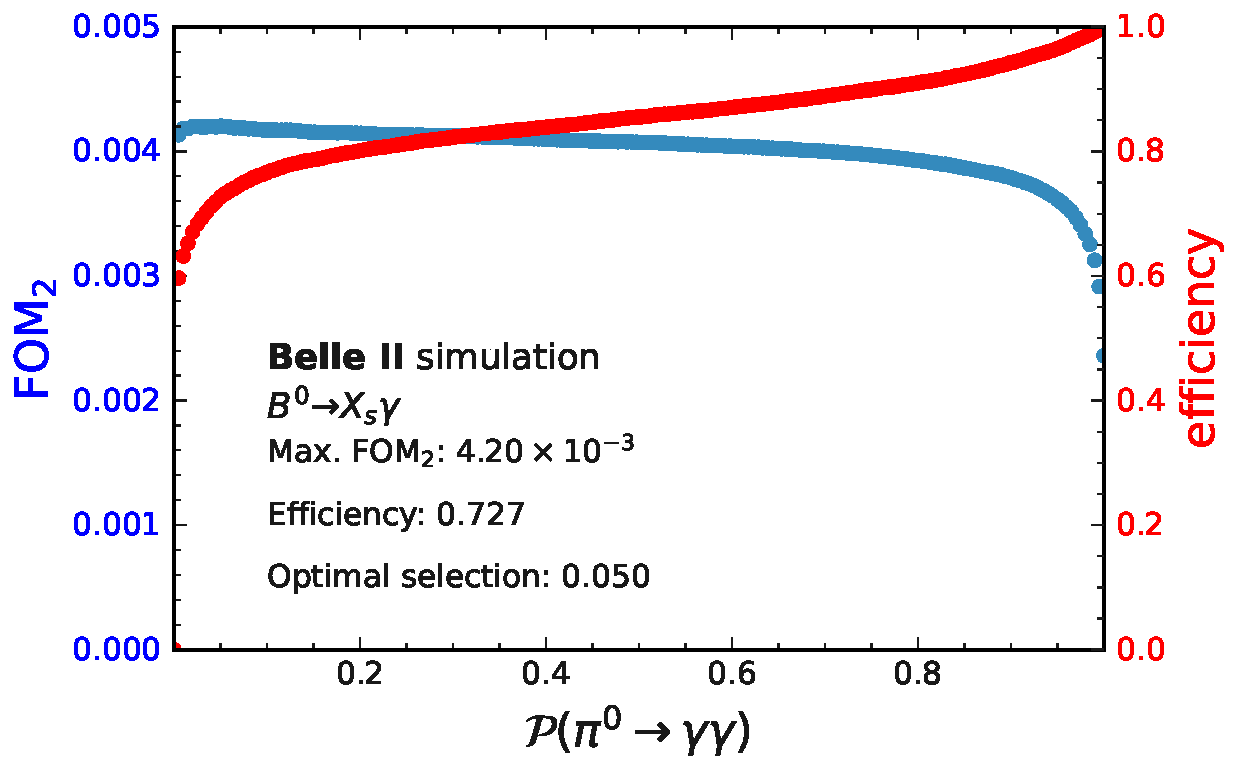
\includegraphics[width=0.3\textwidth]{figures/continuum_suppression/Bz_piVeto_optimisation_punzi.pdf}
        }
    \subcaptionbox{\label{fig:bz_etaveto_optimisation}}{
            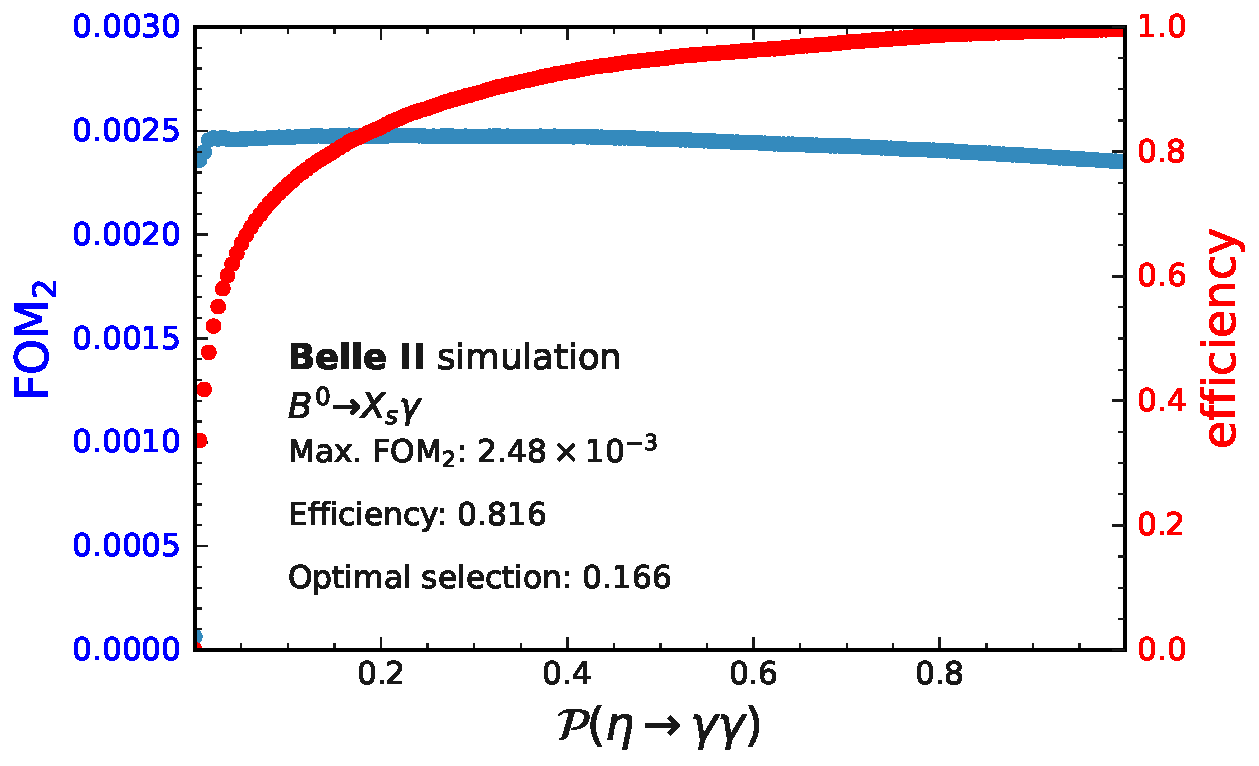
\includegraphics[width=0.3\textwidth]{figures/continuum_suppression/Bz_etaVeto_optimisation_punzi.pdf}
        }
    \caption{\label{fig:selection_optimisations} Optimal selection calculation for observables
    described in \Cref{sec:photon_selection} based on $\mathrm{FOM}_2$ (see \Cref{eq:punzi_fom}).
    For \BptoXsgamma events the tests are shown
    in \Cref{fig:bp_zmva_optimisation,fig:bp_piveto_optimisation,fig:bp_etaveto_optimisation},
    and for \BztoXsgamma in \Cref{fig:bz_zmva_optimisation,fig:bz_piveto_optimisation,fig:bz_etaveto_optimisation}.
    The figures show efficiency and $\mathrm{FOM}_2$ score calculated for 200 selections of \piVeto, \etaVeto and \ZMVA.
    The maximum value of $\mathrm{FOM}_2$, the corresponding selection and efficiency are shown as well.
    }
\end{figure}

The results between \Bp and \Bz modes, as well as using $\mathrm{FOM}_1$ and $\mathrm{FOM}_2$ are consistent, with only marginal differences.
Therefore, due to the model-independance of $\mathrm{FOM}_2$, this figure-of-merit will be the only one discussed henceforth.
At this stage, it is unnecessary to choose the `best' selection, as another simultaneous optimisation will be performed later, together with continuum suppression \BDT output.
\todo[inline]{(see XXX when I optimise)}. 
The main goal is to reduce the sample size to include only relevant data, such that the trained \BDT can make decisions for difficult cases that are not easily distinguishable using simple selection.
Based on \Cref{fig:selection_optimisations}, pre-selections are chosen, which suppress background but retain most of the signal.
The requirement for a loose selection are tailored such that more roughly 75\% of \BtoXsgamma candidates are retained and are shown in \Cref{tab:preselections}.
They are chosen to be no tighter than their optimal selection and preferrably considerably looser.

\begin{table}[htbp!]
    \centering
    \caption{\label{tab:preselections} \todo[inline]{add caption}}
    
    \begin{tabular}{|lr|}
    \hline
    Variable &    Loose selections \\
    \hline
    \ZMVA & $>0.5$ \\
    \piVeto            & $<0.4$ \\
    \etaVeto           & $<0.4$ \\
    
    \hline
    
    $B^+$ mode: $\gamma$ candidate retention efficiency & 75.4\% \\
    $B^0$ mode: $\gamma$ candidate retention efficiency & 76.7\% \\
    \hline
    \end{tabular}

\end{table}

The pre-selections improve the signal-to-background ratio by roughly an order of magnitude.
This can be clearly seen by comparing \Cref{fig:preselected_photons} with \Cref{fig:spectrum_after_reco}.
The scale at which \BtoXsgamma signal \MC scaled differs at about a factor of 10, meaning that the background reduced by approximately that amount due to these selections.


\begin{figure}[htbp!]
    \centering
    \subcaptionbox{\label{fig:bp_preselected_photons}}{
        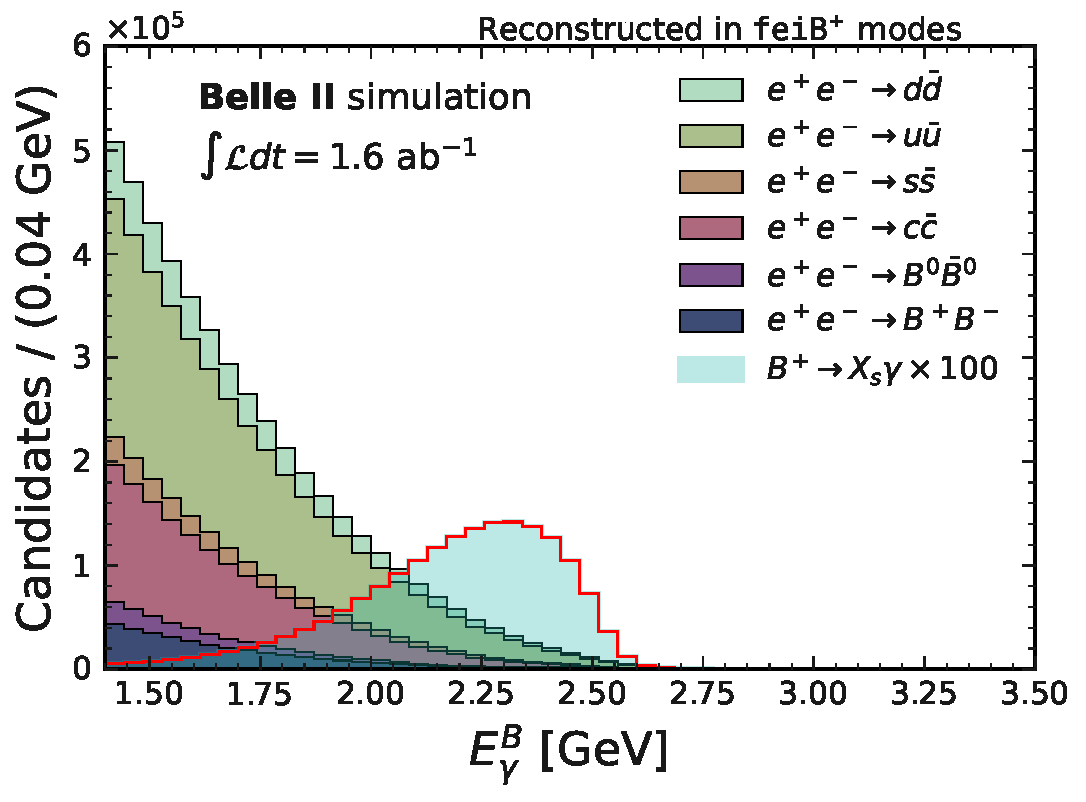
\includegraphics[width=0.395\textwidth]{figures/continuum_suppression/Bp_tagged_background_preselection.pdf}
    }
    \subcaptionbox{\label{fig:bz_preselected_photons}}{
        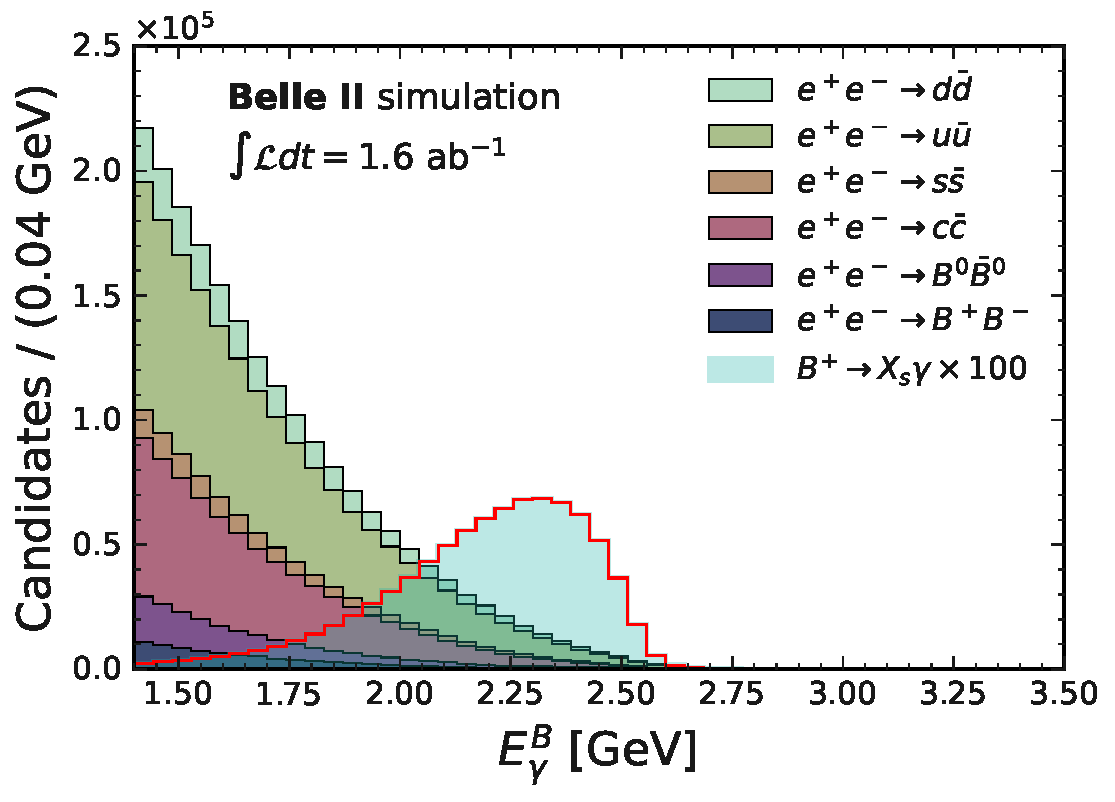
\includegraphics[width=0.395\textwidth]{figures/continuum_suppression/Bz_tagged_background_preselection.pdf}
        }
    \caption{\label{fig:preselected_photons} \BtoXsgamma spectrum in generic \MC after pre-selection for training the continuum suppression \BDT classifier.
    Overlaid are events from signal \MC where the photon comes from \BtoXsgamma, multiplied by a scaling factor.
    Compared to \Cref{fig:spectrum_after_reco}, the effectiveness of background suppression so far is apparent.
    These figures may include multiple tag entries per event.
    }
\end{figure}

Finally, many combinatorial tag-side candidates in \BB events may still appear contribute to the analysis at this stage.
A more detailed definition for a `well-reconstructed' tag will be explored later 
\todo[inline]{add later}.
At this stage, it is sufficient to acknowledge the fact that the vast majority of correctly reconstructed tag-side candidates is expected to lie $\Mbc>5.27~\gevcc$.
Therefore, this requirement is also adopted for studies and training in \Cref{sec:continuum_features}--XXX
\todo[inline]{add X}.

\subsection{Continuum suppression strategy}\label{sec:continuum_features}

$B$ factory experiments and Belle II have a large selection of observables that can be utilised for continuum suppression and are suitable to be input as variables to a \BDT.
These observables combine describe the event-topology or particles in the event and are optimised to provide separation between \BB and \qqbar events.
There are two caveats that have to be kept in mind for the \BtoXsgamma analysis:
\begin{itemize}
    \item Generally, \BtoXsgamma event-topology may be different compared to \BB events. 
    \BtoXsgamma decays have a single jet-like $X_s$ system (while the other $B$ meson decays hadronically).
    This leads to a somewhat middle-case between a generic-\BB event and a \epem\ra\qqbar event, as it was illustrated in \Cref{fig:continuum_schematic}.
    \item Many of these observables contain momenta, angles or other parameters of some (or even all) particles in the event -- including the $X_s$ system and the photon.
    This may lead to a bias to the spectrum of $X_s$ system.
    Furthermore, even relatively small biases, over many different different training features used, may be learnt by the \BDT and introduced to the spectrum.
    \item Some of the features may perform differently in real-data compared to simulation, due to unexpected differences in alignment, calibration or background distributions.
    As we use simulated data sets to train a \BDT in this analysis, such a comparison is crucial.
\end{itemize}
Given the mentioned points, it is important to test that observables used for the training provide adequate separation between \BtoXsgamma and \qqbar, while no bias is introduced to the photon energy spectrum.
Furthermore, this has to be well-represented in data.

In this analysis, the following observable categories are considered for separation between \epem\ra\qqbar and \BtoXsgamma:
\begin{itemize}
    \item Various thrust-based observables (\Cref{sec:thrusts});
    \item Sphericity and aplanarity (\Cref{sec:sphericity_aplanarity});
    \item Harmonic moments (\Cref{sec:harmonic_moments});
    \item Fox-Wolfram moments (\Cref{sec:fox_wolfram_moments});
    \item Modified Fox-Wolfram moments (\Cref{sec:modified_fox_wolfram_moments});
    \item CLEO cones (\Cref{sec:cleo_cones});
    \item Angular tag-$B$ meson observables (\Cref{sec:angular_features});
    \item Tag-$B$ meson vertex observables (\Cref{sec:vertex_features});
    \item Flavour tagger output for the tag-$B$ meson(\Cref{sec:flavour_tagger_outputs});
\end{itemize}

In total, this provides 81 potential training features that are tested to be unbiased and adequately described in simulation.
The tests use a metric of \textit{total divergence to the average} (often called \textit{Jensen-Shannon distance}) \cite{Lin:1991abc},
which is used to quantitatively evaluate the similarity between two distributions.
The Jensen-Shannon distance is bounded by 1 for two given probability distributions, $\mathbb{X}_1$ and $\mathbb{X}_2$:
\begin{equation}\label{eq:js_distance}
    0\leq\mathrm{JSD}(\mathbb{X}_1||\mathbb{X}_2) \leq1,
\end{equation}
where exactly similar distributions have a score of 0, and the score tends towards 1 when the distributions are highly-different.

Two tests are performed:
\begin{itemize}
    \item \textbf{Test 1}: $\mathbf{\EB,~\Estar~and~tag\mbox{-}side~\Mbc~bias~test}$:
    to ensure that the classifier does not indirectly select particular $X_s$ or tag-side $B$ channels,
    each tested potential training feature is separated into 5 equally populated regions (\texorpdfstring{slices}) of \BtoXsgamma events in signal \MC.
    For this test, \BptoXsgamma and \BztoXsgamma are merged.
    In each of these regions, the distribution of \EB, \Estar and \Mbc is compared.
    The Jensen-Shannon distance is required to not be larger than 6\% between any two given slices of a training feature.
    The requirement to pass \textbf{Test 1} has been chosen by observing the typical values of the agreement shown by the tested unbiased distributions.
    If this requirement is not passed by at least one of the distributions (\EB, \Estar or \Mbc), the feature is excluded from the list of final \BDT training features.
    \item \textbf{Test 2}: $\mathbf{\epem\ra\qqbar~data\mbox{-}simulation~similarity~test}$:
    to ensure that simulations adequatly describe the data sets that we aim to suppress.
    This test is only performed if \textbf{Test~1} is passed.
    As this is a blinded analysis, off-resonance data samples are used, which only contain \epem\ra\qqbar events.
    In this case, the Jensen-Shannon distance is calculated between 
    the area-normalised distribution of a training feature in off-resonance data set,
    and the area-normalised distribution of a training feature in \epem\ra\qqbar simulation.
    The metric is required to be no more than 15\%.
    The looser requirement is adopted here, due to the fact that some difference is expected between the distributions,
    as the collision energy in off-resonance data set is different to the one in on-resonance simulation that is used in this analysis.
    Furthermore, an overall smaller off-resonance data set ($\sim19~\invfb$, see \Cref{sec:data_samples}) may have certain difference due to poissonian fluctuations.
\end{itemize}

The tested distributions have the selections from \Cref{sec:preselection} included, except for the case of off-resonance dataset, where the $\Mbc>5.27~\gevcc$ requirement is lifted.
For every event, when more than one tag-side candidate $B$ candidate exists, a random one is picked.
\textbf{Test~1} with exact definitions for the tested variable categories are shown in \Cref{sec:appendix_continuum_features}.



